\chapter{MindSpore介绍}

\footnote{MindSpore的安装和使用本可放置在\S\ref{sec:local-env}中,但为了增加对MindSpore的介绍,同时为表对华为提供计算资源的支持,特将MindSpore相关内容编撰成本章。在我们的实验中,同学们在Pytorch或MindSpore其中之一完成实验即可。但目前,实验指导书中的内容仍以Pytorch为主,仅在实验一\S\ref{chapter:task1}中介绍了使用MindSpore完成实验的方法,如需使用MindSpore完成其余实验,同学们需自行查阅资料、阅读官网文档。}
华为开源自研AI框架{\CJKfontspec{等线}昇}思MindSpore,是一个全场景深度学习框架,旨在实现易开发、高效执行、全场景覆盖三大目标。自动微分、并行加持,一次训练,可多场景部署。支持端边云全场景的深度学习训练推理框架,主要应用于计算机视觉、自然语言处理等AI领域。

正如第一章\S\ref{sec:huawei-cloud-usage}介绍,本课程得到了华为云的大力支持,因此本课程也鼓励同学们积极使用华为自研的国产AI框架,积极反馈或贡献,为我国人工智能发展贡献力量。具体到本课程的实验,我们将像使用Pytorch那样使用MindSpore。



\section{整体介绍}

华为AI致力于构建业界最强的AI算力平台,使能千行百叶的智能化转型。华为AI的整体框架如图\ref{fig:mindspore-whole-picture}所示,其中可以看到我们在\S\ref{sec:huawei-cloud-usage}中介绍的华为ModelArts平台和MindSpore框架所处的位置。
\begin{figure}[htbp]
	\centering
	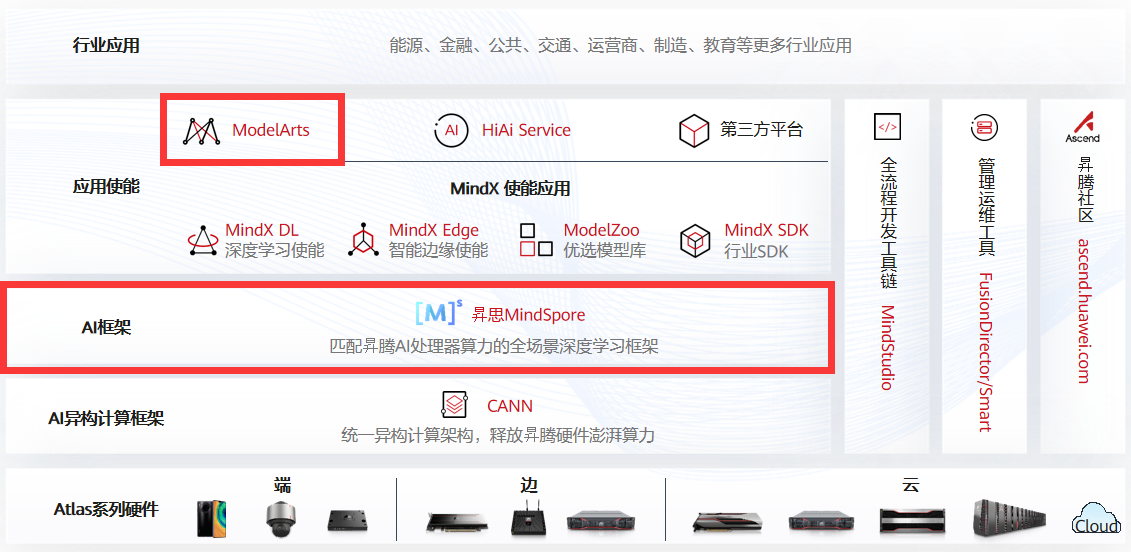
\includegraphics[width=1\textwidth]{figures/mindspore-whole-picture.png}
	\caption{caption:mindspore-whole-picture}
	\label{fig:mindspore-whole-picture}
\end{figure}

MindSpore框架拥有全场景AI计算能力,图\ref{fig:mindspore-ai-architecture}展示了MindSpore全场景AI计算框架架构图,其包含了AI计算所需的各个组件,从软件到硬件,从网络模型、API表达层、编译优化层到底层各种计算资源硬件和其使用框架,均包含在MindSpore中。

\begin{figure}[htbp]
	\centering
	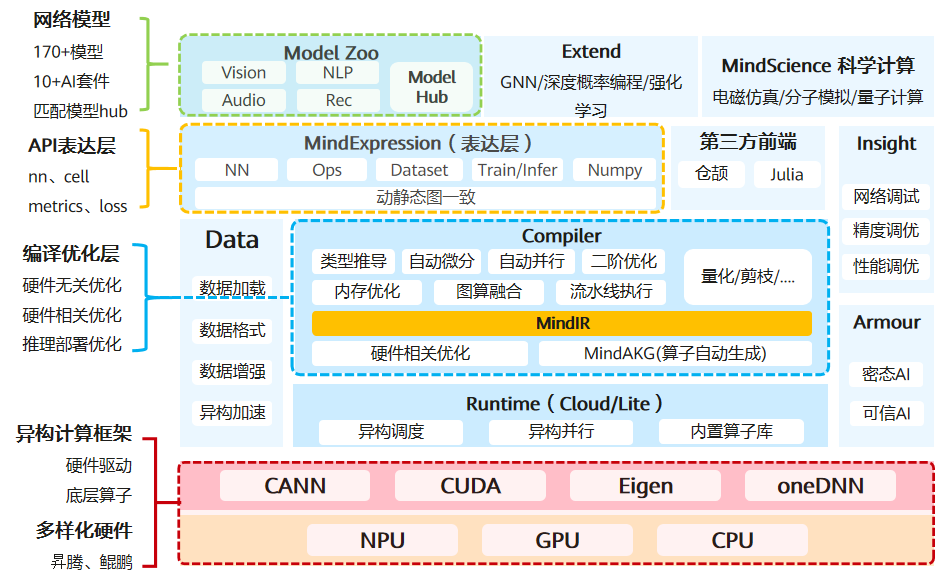
\includegraphics[width=1\textwidth]{figures/mindspore-ai-architecture.png}
	\caption{caption:mindspore-ai-architecture}
	\label{fig:mindspore-ai-architecture}
\end{figure}


MindSpore 架构具有如下特点:
\begin{itemize}
    \item 用户态易用;
    \item 运行态高效;
    \item 部署态灵活;
\end{itemize}

MindSpore 具有如下特性:
\begin{itemize}
    \item 自动并行:通过自动并行机制、数据pipeline处理等手段降低超大模型训练门槛。
    \item AI+科学计算:支持AI+科学计算的高阶/高纬、多范式编程。
    \item 通用计算+DSA:通过图算融合对性能进行优化,自动算子生成技术简化异构( DSA )编程,发挥多样性算力的性能。
    \item 端边云统一的可信架构:解决企业级部署和可信的挑战。
\end{itemize}


MindSpore包含了MindExpress、MindCompiler、MindSpore Runtime、MindData等多个子系统,在实验指导书中不再赘述,有兴趣了解的同学可以参考助教分享的演示文稿。


\section{MindSpore安装}

安装过程也与Pytorch的安装类似,具体而言,打开\url{https://www.mindspore.cn/install},选择合适的版本、平台等后,按照网站的指示安装即可。

\begin{figure}[htbp]
	\centering
	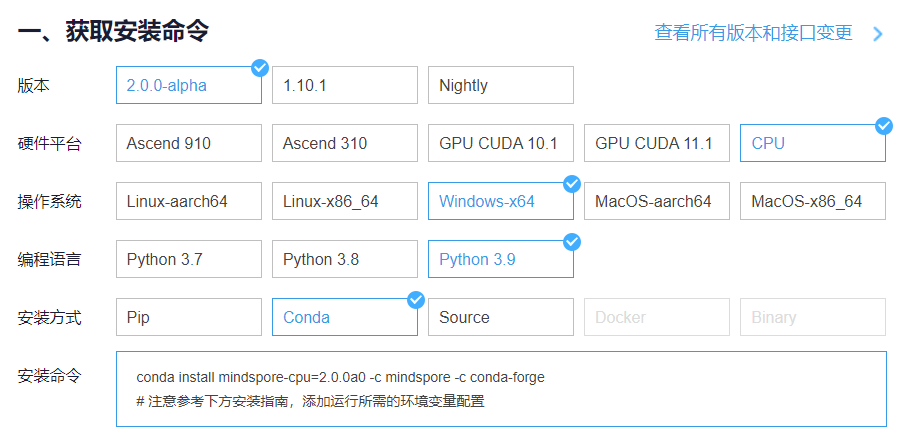
\includegraphics[width=1\textwidth]{figures/mindspore-install.png}
	\caption{caption:mindspore-install}
	\label{fig:mindspore-install}
\end{figure}

\section{社区资源}
\begin{itemize}
    \item {\CJKfontspec{等线}昇}腾开发者社区: \url{https://hiascend.com}
    \item {\CJKfontspec{等线}昇}腾论坛: \url{https://www.hiascend.com/forum/}
    \item MindSpore开源社区:  \url{https://www.mindspore.cn/}
    \item ModelArts社区:  \url{https://bbs.huaweicloud.com/forum/forum-718-1.html}
    \item Gitee仓库: \url{https://gitee.com/mindspore}
\end{itemize}



\vspace{3em}
至于MindSpore的使用,我们将在对应实验章节内进行介绍。